\chapter{Introduction} \label{chapt:Introduction}
People recognise concepts, rules, restraints, and information as `knowledge'. Data is often treated as the basis of constructing knowledge. Traditionally, data mining and knowledge discovery was performed manually. As time passed, the amount of data in many systems grew to larger than terabyte size, and could no longer be maintained manually, which brought the idea of machine learning and data mining, also formed a part of artificial intelligence.

%Raw data can be structured, which means it resides in relational databases, like the information stored in a university's enrolment database. It can also be semi-structured, that does not conform with the formal structure of data models associated with relational databases or other forms of data tables, for instance, textual, graphical and image data. 

The process of knowledge discovery has been widely discussed since late $20^t^h$ century and focused on acquiring knowledge that is accurate and precise. The latter focus emphasises the execution efficiency of the algorithms. This may be achieved by adopting a more efficient data structure or having a faster processing mechanism.

\section{Big data and Data Mining}

Big data consists of large datasets that often exceed the collection, utilisation, management, and processing capabilities of humans within acceptable times. The size of big data often may vary. As in 2012, the size of a single dataset ranges from a few terabytes (TB) to tens of petabytes (PB) \cite{wiki:bigdata}.

Doug Laney \cite{bigdata}, an analyst at META Group (now Gartner) in 2001, articulated the challenges and opportunities for data growth have three directions: volume, variety, and velocity, collectively referred to as ``3V'' or ``3Vs'' \cite{bigdata}. Gartner and most of the companies in the big data industry today continue to use 3V to describe big data. Gartner revised the definition of big data in 2012 as: ``Big data is a large, high-speed and changeable information asset that requires new ways of processing to enable better decision making, insight and optimisation.'' In addition, there is the fourth V has been recently defined outside the 3V: veracity, to make an up-to-date definition: ``4V''. The ``4V'' definition is explained as following:

\begin{itemize}
    \item \textbf{Volume}. Organisations collect data from a variety of sources, including business transactions, social media and information from sensor or machine-to-machine data. In the past, storing it would have been a problem – but new technologies (such as Hadoop) have eased the burden.
    
    \item \textbf{Velocity}. Data streams in at an unprecedented speed and must be dealt with in a timely manner. RFID tags, sensors and smart metering are driving the need to deal with torrents of data in near-real time.
    
    \item \textbf{Variety}. Data comes in all types of formats – from structured, numeric data in traditional databases to unstructured text documents, email, video, audio, stock ticker data and financial transactions.
    
    \item \textbf{Veracity}. Big data veracity refers to the biases, noise and abnormalities, ambiguities, latency in data.
    
\end{itemize}

Big data must be statistically collected, compared, and parsed to a computer to produce objective results. The United States started to emphasise their research on big data in 2012. In the same year, President Obama invested 200 million dollars in the development of big data analytical projects, and emphasised that big data will be the future petroleum. 

As we all know, big data is not simply a fact of big data, but the most important is how to analyse big data. We can only get intelligent, in-depth and valuable information through data analysis. There are several methodologies that are common in big data analysis:

\begin{enumerate}

    \item \textbf{Visualisation}. As the target audience of big data analysis report may not be statistics or computer science professionals, it is very important to ensure that the information provided are relevantly direct and understandable. This brings visualisation in the first priority, because visualisation can intuitively present big data features and can be understand is as simple and straightforward as reading a picture.
    
    \item \textbf{Data mining algorithms}. The theoretical core of big data analysis is data mining algorithms. Various data mining algorithms based on different data types and formats can present the characteristics of the data more scientifically. The algorithms can usually achieve good efficiency which can significantly improve the cost of big data analysis.
    
    \item \textbf{Prediction}. One of the most important goals of big data analysis is to make predictions. After the characteristics are extracted from big data, data scientist can build a model based on these characteristics and predict the future trends. 
    
    \item \textbf{Big data management}. Big data analysis is inseparable from keeping the integrity and quality of input data. High-quality data and an effective data management will be beneficial in both academic research and commercial development, to ensure the authenticity and value of the results.
    
\end{enumerate}

Data mining, also as known as Knowledge Discover in Database (KDD), is the process of extracting information that is hidden from the prior art, but is potentially useful, from a large number of incomplete, noisy, fuzzy, and random practical data. This definition includes several layers of meaning: the data source must be real, large, and noisy; the knowledge that is of interest to users; the knowledge found is acceptable, understandable, and usable.

In the next section, we are going to look at data stream mining by defining data stream first then discuss some unique characteristic of data stream and how to make proper analysis on it.

\section{Data Stream Mining}

Data stream is ubiquitous in our lives. The telephone communication records, social media use, retail sales transactions and even the real-time stock exchange information are all data streams.

What is a data stream? We can understand that the data in these situations mentioned above have a common feature, that is, infinity. In addition to endless incoming data, think about the retail transactions and stock exchange records, they both have a very fast updating speed, which makes the timing critical for data stream analysis. The data first seen in the data stream could be expired after new data arrives. 

To understand and analyse the characteristics of the data stream, we naturally think, can we apply the traditional data mining method to data stream? As several mature data mining methods have developed during the last decades, data source is stored in flat files, relational databases, transactional databases, etc. These methods (such as OLAP) are built on top of data that has been saved statically and not updated frequently, for example, a data warehouse. Furthermore, some of our methods requires more than one access to the data. However, it is almost impossible to store data stream because of its infinite size and consistent updates. Aim to process a special type of data like data stream, it is better to scan the data once or a constant number of times but not the entire data stream to reduce the memory use. 

\subsection{Association Rule Mining}
For the successful existence of any business, discovering underlying patterns in data is considered essential. As a result, several pattern mining algorithms were developed to discover hidden data and make assumptions, which formed a part of artificial intelligence. These algorithms are able to find either the features which occur together or those are somehow correlated. 

What does the value of one feature tell us about the value of another feature? For example, people who buy nappies are likely to buy baby powder. Or we can rephrase the statement by saying: if (people buy nappies), then (they buy baby powder). Note the if, then rule. This does not necessarily mean that if people buy baby powder, they buy nappies. In General, we can say that if condition A tends to B it does not necessarily mean that B tends to A. The relationship between nappies and baby powder can be treated as an association rule, that is the interesting patterns we aim to mine from data streams.

Section~\ref{chapt:RelatedWorks} will have more discussion on the techniques which have been widely researched and used on data stream mining especially on association rule mining. To better mining significant patterns out from data stream, we will address out motivation in the next section.


\section{Motivation}

One of the most researched fields for data stream is mining significant patterns out of data stream. Current research in data stream pattern mining relies on using minimum or maximum support thresholds to derive the association rules~\cite{kingfisher}, which comes with many drawbacks such as not considering the statistical significance of patterns. Thus, these work may find many frequent patterns that are spurious - contains values that appear together by chance rather than having a strong correlation. To solve this drawback, Webb et al. \cite{ssi,topk} proposed and defined self-sufficient itemsets to produce more `interesting' rules. Those are itemsets having a frequency that cannot be explained solely by the frequency of their subsets or supersets. It has been shown that itemsets derived using minimum support that does not also satisfy the definition of self-sufficient itemsets are unlikely to produce interesting rules. Given the infinite growth of data streams, we require the association rule mining algorithms to be workable on a data stream. 


While a large number of papers discussed mining interesting association rules from data streams, the non-stationary distributions problem has not been as widely dealt with in the pattern mining research domain. Changes in the underlying distribution may lead to changes in the relevant pool of itemsets over time, which will reduce the correctness of interesting rules mined. This is known as the concept drift problem. In this section, we look at official retail data from Stats NZ~\cite{statsnz} which helps illustrate concept drift problems in data stream mining.

Figure \ref{fig:retail1} and \ref{fig:retail2} below are retail sales data in two different quarters: December 2017 to March 2018 and March 2018 to June 2018. It is very interesting to see that people buy significantly different goods in these two quarters. For instance, we look at sales of grocery, liquor and tobacco product from Quarter 1 2018 to Quarter 2 2018. The figures show us that sales went down in the first quarter of 2018 but went rapidly up during the second quarter. This kind of distribution changes bring the challenge of using a static model to mine patterns for a entire data stream. Obviously, changes need to be separately considered to ensure the accuracy of data stream pattern mining. 

\begin{figure}[H]
    \centering
    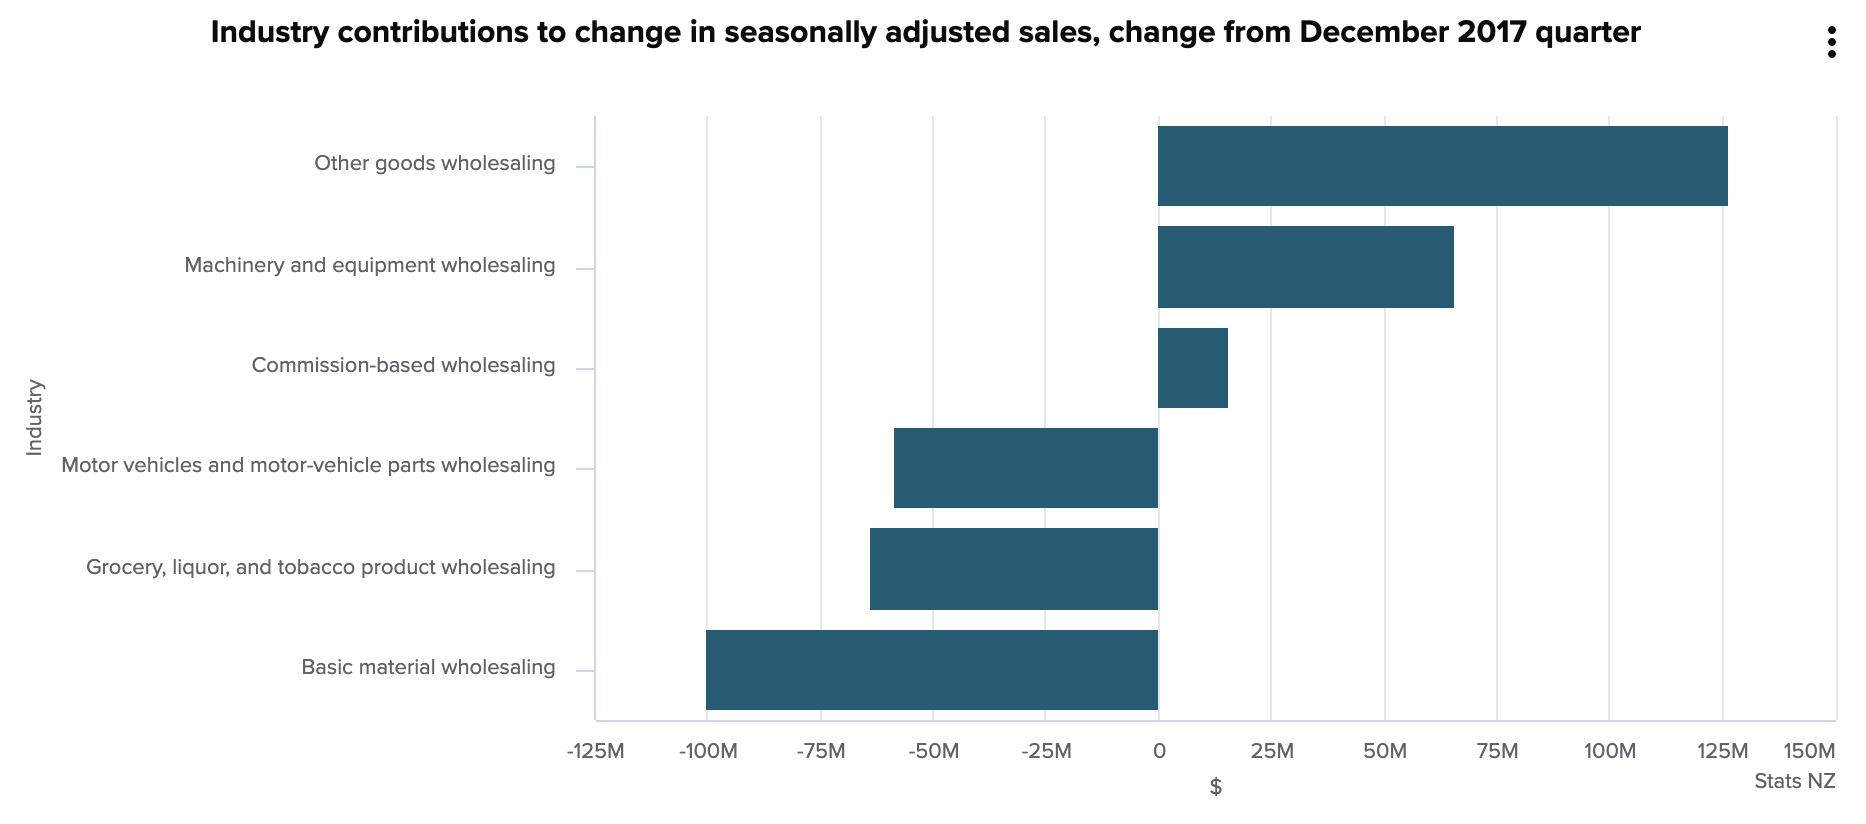
\includegraphics[width=\textwidth]{Introduction/1217to0318.png}
    \caption{NZ Retail data from 12-2017 to 03-2018 \cite{statsnz}}
    \label{fig:retail1}
\end{figure}

\begin{figure}[H]
    \centering
    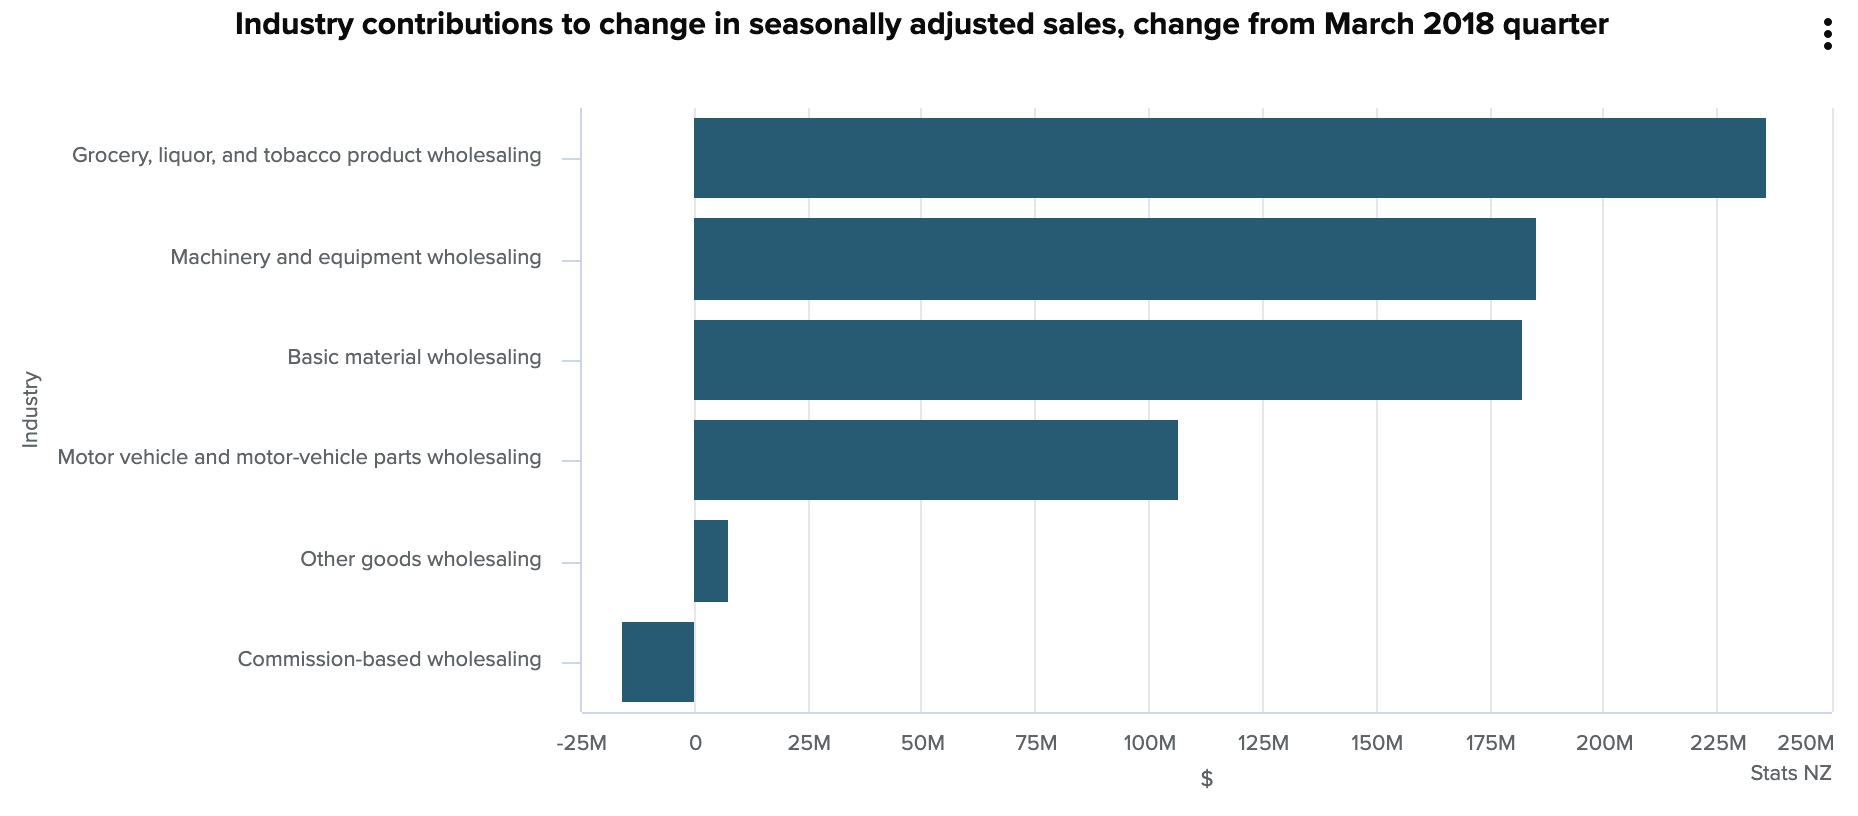
\includegraphics[width=\textwidth]{Introduction/0318to0618.png}
    \caption{NZ Retail data from 03-2018 to 06-2018 \cite{statsnz}}
    \label{fig:retail2}
\end{figure}



%Small work around example of regional drift 

Currently when a change is detected by the concept drift detector, the entire existing set of rules previously found are discarded and we re-mine the rules from the new data in the data stream. This is an inefficient method since there is a possibility that only a small portion of the rules have changed and discarding and re-mining entire sets to discover small changes is not ideal. There is also the problem of setting a proper interval value to discard and re-mine. If we discard and re-mine too frequently, the running cost will be high. One the other hand, if we discard and re-mine too infrequently, we risk not picking up the correct rules within the time-frame. For example, using supermarket basket analysis data, consider the situation where the supplier for Cheerios had suddenly stopped supplying Cheerios to the supermarket. As a consequence, future transactions will not contain Cheerios and this leads to a concept drift. If we discarded and re-mined at this time, the patterns containing Cheerios will be lost. If Cheerios immediately starts to restock after we re-mined, we are not able to pick up the patterns related to Cheerios again. Therefore, in this case, the disappearance of Cheerios could be identified as a regional drift. Mining regional drifts allow us to better adapt to the intricate changes in the patterns over time. 

\section{Research Questions and Objectives}
In this dissertation we study adaptive association rule mining in data streams. Adaptive association rule mining refers to updating learning models to react to the presence of changes. The prior sections list the background and motivations, the specific research questions that we look at are:

\subsection{Research Questions}
\begin{enumerate}
\item Why pure ``support-confidence'' framework is not sufficient to solve some real-world association rule mining problems?

\item Can we propose a working approach that facilitates the discovery of self-sufficient itemset accurately and efficiently in data streams.

\item Can we define and introduce the problem of detecting concept drift in self-sufficient itemset mining in data streams?

\item Can we develop a self-sufficient itemset mining technique that also detects and adapts to different kinds of concept drifts accurately and efficiently in data streams?
\end{enumerate}

\subsection{Objectives}
This dissertation focuses on developing algorithms that overcome the drawbacks of the ``support-confidence'' mining technique and adapt to different kinds of concept drifts to effectively acquire and learn knowledge from data streams. Our objectives are:

\begin{enumerate}
\item To address drawbacks of the pure ``support-confidence'' framework and compare it with improved techniques such as Self-Sufficient itemset.

\item To establish adaptive self-sufficient itemset mining using not only the pure support and confidence of items but also their associations with each other.

\item To develop a novel technique that detects and adapts to abrupt, gradual and regional concept drifts that occurs in data stream.

\item To develop an algorithm that solves the problem of mining self-sufficient itemset in an online mode along with concept drift adaption.
\end{enumerate}

\section{Contributions}

The main contributions made by this dissertation are:


\begin{enumerate}
\item I review work from several disciplines which may be of relevance to the present sub-ject of inquiry, and provide commentary on how the findings from these disciplines may be useful (Section~\ref{chapt:RelatedWorks}).

\item I provide a framework for mining self-sufficient itemset mining using not only the pure support and confidence of items but also their associations with each other. With this framework as a reference template, future work in this domain should be able to proceed more adaptive and accurate. (Section~\ref{chapt:ASSIM}).

\item By applying this framework to transactional data streams, I am able to detects and adapts to abrupt, gradual and regional concept drifts that occurs during the self-sufficient itemset mining process and adapt to those drifts. This allows future self-sufficient itemset mining achieve more accurate and stable results. (Section~\ref{chapt:ASSIM})

\end{enumerate}


\section{Structure of Dissertation}

This dissertation is structured into the following chapters:

\begin{itemize}
    
    \item \textit{Section~\ref{chapt:Introduction} Introduction}\newline
    We provide the reader with the relevant background to understand this dissertation.

    \item \textit{Section~\ref{chapt:RelatedWorks} Related Works}\newline
    We introduce relevant research in association rule mining, self-sufficient itemset, and concept drift mining. In particular, we detail seminal research and review the overall state of the current research. We also review the difference in the works pertaining to the traditional ``support-confidence'' technique versus the self-sufficient itemset discovery framework.
    
    \item \textit{Section~\ref{chapt:ASSIM} Self-sufficient Itemset Stream Mining}\newline
    We propose our Adaptive self-sufficient Itemset Miner (ASSIM) framework, discuss how its components interacts with each other, and explain how ASSIM improves the mining process of self-sufficient itemsets.
    
    \item \textit{Section~\ref{chapt:Experiments} Experiments}\newline
    We perform several experiments on evaluating the key components of ASSIM by comparing their computational costs, precision \& recall, and other important measures.
    
    \item \textit{Section~\ref{chapt:Conclusion} Conclusion}\newline
    We conclude the work, point out future directions and add some final reflections and remarks.
\end{itemize}

